\documentclass[12pt,a4paper]{article}
\usepackage[top=2.5cm,bottom=2.5cm,left=2.5cm,right=2.5cm,headheight=15pt]{geometry}
\usepackage{amsmath,amssymb}
\usepackage{tikz}
\usetikzlibrary{shapes,arrows,arrows.meta,positioning,calc,backgrounds,fit,matrix}
\usepackage{booktabs,array,longtable,tabularx,multirow}
\usepackage{xcolor}
\usepackage{enumitem}
\usepackage{fancyhdr}
\usepackage{titlesec}
\usepackage{mdframed}
\usepackage{tcolorbox}
\tcbuselibrary{skins,breakable}
\usepackage{hyperref}

%% ---- Colors ----
\definecolor{folblue}{RGB}{0,82,165}
\definecolor{lightblue}{RGB}{220,235,255}
\definecolor{darkorange}{RGB}{180,70,0}
\definecolor{lightorange}{RGB}{255,235,210}
\definecolor{darkgreen}{RGB}{20,110,20}
\definecolor{lightgreen}{RGB}{200,240,205}
\definecolor{darkred}{RGB}{150,20,20}
\definecolor{lightred}{RGB}{255,210,210}
\definecolor{lightgray}{RGB}{242,242,242}

%% ---- tcolorbox styles ----
\newtcolorbox{qbox}[2][]{enhanced,breakable,
  colback=lightorange,colframe=darkorange,arc=4pt,
  title={\textbf{#2}},fonttitle=\bfseries\color{white},
  attach boxed title to top left={yshift=-2mm,xshift=4mm},
  boxed title style={colback=darkorange,arc=3pt},#1}

\newtcolorbox{solbox}[2][]{enhanced,breakable,
  colback=lightblue,colframe=folblue,arc=4pt,
  title={\textbf{#2}},fonttitle=\bfseries\color{white},
  attach boxed title to top left={yshift=-2mm,xshift=4mm},
  boxed title style={colback=folblue,arc=3pt},#1}

\newtcolorbox{keybox}[2][]{enhanced,breakable,
  colback=lightgreen,colframe=darkgreen,arc=4pt,
  title={\textbf{#2}},fonttitle=\bfseries\color{white},
  attach boxed title to top left={yshift=-2mm,xshift=4mm},
  boxed title style={colback=darkgreen,arc=3pt},#1}

\newtcolorbox{algobox}[2][]{enhanced,breakable,
  colback=lightgray,colframe=gray!60,arc=4pt,
  title={\textbf{#2}},fonttitle=\bfseries,
  attach boxed title to top left={yshift=-2mm,xshift=4mm},
  boxed title style={colback=gray!60,arc=3pt},#1}

\newtcolorbox{warnbox}[2][]{enhanced,breakable,
  colback=lightred,colframe=darkred,arc=4pt,
  title={\textbf{#2}},fonttitle=\bfseries\color{white},
  attach boxed title to top left={yshift=-2mm,xshift=4mm},
  boxed title style={colback=darkred,arc=3pt},#1}

%% ---- Page style ----
\pagestyle{fancy}\fancyhf{}
\lhead{\color{folblue}\textbf{Symmetric/Asymmetric \& Block/Stream Ciphers --- CSE 717 InfoSec}}
\rhead{\color{folblue}Exam: 17 Jun 2026}
\cfoot{--- \thepage\ ---}
\renewcommand{\headrulewidth}{0.4pt}

%% ---- Section style ----
\titleformat{\section}{\large\bfseries\color{folblue}}{}{0em}{}[\titlerule]
\titleformat{\subsection}{\normalsize\bfseries\color{darkorange}}{}{0em}{}

\begin{document}

\begin{center}
{\LARGE\bfseries\color{folblue} CSE 717 --- Information Security}\\[4pt]
{\large\bfseries Topic 3: Symmetric vs Asymmetric \& Block vs Stream Ciphers}\\[2pt]
{\large Complete Past Paper Solutions: 2020--2024}\\[6pt]
{\normalsize Source: general security knowledge (no-source cheat sheet --- Lc\#1 pp.25--28 and Lc\#7 p.12 are title-only slides with no body text)}\\[2pt]
{\normalsize\color{darkred}\textbf{Every Topic-3 question 2020--2024 included. Zero omissions.}}
\end{center}

\tableofcontents
\newpage

%% ==========================================
\section*{Quick Reference --- Cheat Sheet}
%% ==========================================

\begin{warnbox}{No-source cheat sheet --- like Topics \#13 / \#14}
None of Lc\#1--11 contain body text on: essential ingredients of a symmetric cipher, block vs stream cipher, classical Feistel structure, or public-key cryptosystem elements/roles. The slides only show title pages ("How Cryptography Works with Public and Private Key?", "Why Symmetric Algorithms Are Less Vulnerable"). Everything below is standard cryptography knowledge (Stallings) memorized as a cheat sheet.
\end{warnbox}

\begin{algobox}{1. Essential Ingredients of a Symmetric Cipher (5 components)}
\begin{enumerate}[noitemsep]
  \item \textbf{Plaintext:} the original, readable message/data fed into the algorithm.
  \item \textbf{Encryption algorithm:} performs substitutions/transformations on the plaintext.
  \item \textbf{Secret key:} an independent value that controls the exact substitutions/transformations --- both sender and receiver must share it via a secure channel.
  \item \textbf{Ciphertext:} the scrambled output, depends on the plaintext \emph{and} the key.
  \item \textbf{Decryption algorithm:} the encryption algorithm run in reverse, using the same secret key, to recover the plaintext.
\end{enumerate}
\end{algobox}

\begin{algobox}{2. Block Cipher vs Stream Cipher (one-line difference)}
\begin{itemize}[noitemsep]
  \item \textbf{Block cipher:} encrypts a fixed-size \textbf{block} of plaintext (e.g.\ 64/128 bits) at a time, using the same key for each block (e.g.\ DES, AES).
  \item \textbf{Stream cipher:} encrypts plaintext \textbf{one bit/byte at a time}, combining it with a pseudorandom keystream (typically via XOR) as the data streams in (e.g.\ RC4).
  \item \textbf{Memory aid:} block = "batch processing", stream = "one unit at a time, on the fly".
\end{itemize}
\end{algobox}

\begin{algobox}{3. Classical Feistel Cipher Structure}
A Feistel network splits each plaintext block into two halves $L_i, R_i$ and applies $n$ rounds. In each round $i$:
\[
L_i = R_{i-1}, \qquad R_i = L_{i-1} \oplus F(R_{i-1}, K_i)
\]
where $F$ is a round function and $K_i$ is the round subkey (derived from the main key via a key schedule).
\begin{itemize}[noitemsep]
  \item Decryption uses the \emph{same} structure with subkeys applied in \textbf{reverse order} --- the same hardware/software can do both encryption and decryption.
  \item This is the structure underlying \textbf{DES} (see Topic \#13 cheat sheet for the full diagram with $f$-function, XOR, and swap boxes per round).
\end{itemize}
\end{algobox}

\begin{algobox}{4. Public-Key Cryptosystem: Elements \& Key Roles}
\textbf{Six elements} of a public-key cryptosystem:
\begin{enumerate}[noitemsep]
  \item \textbf{Plaintext} --- the readable input message.
  \item \textbf{Encryption algorithm} --- performs transformations on the plaintext.
  \item \textbf{Public key \& private key} --- a mathematically linked pair; one for encryption/verification, the other for decryption/signing.
  \item \textbf{Ciphertext} --- the scrambled message produced by the algorithm + key.
  \item \textbf{Decryption algorithm} --- accepts the ciphertext and the matching key to recover the plaintext.
\end{enumerate}
\textbf{Roles of the keys:}
\begin{itemize}[noitemsep]
  \item \textbf{Public key:} freely distributed; used by anyone to \emph{encrypt} a message for the owner, or to \emph{verify} the owner's digital signature.
  \item \textbf{Private key:} kept secret by the owner; used to \emph{decrypt} messages encrypted with the matching public key, or to \emph{create/sign} a digital signature.
\end{itemize}
\end{algobox}

\newpage
%% ==========================================
\section{2024 --- Q1(a): Symmetric vs Asymmetric Crypto (3 marks) --- cross-reference}
%% ==========================================

\begin{qbox}{Question --- 2024 Q1(a)}
Briefly describe symmetric and asymmetric cryptography with an example. Point out the reason why asymmetric cryptography is useful for e-commerce. \hfill [3]
\end{qbox}

\begin{solbox}{Answer --- already fully solved under Topic 2}
This question is bundled with Topic 2 (Security Fundamentals) in 2024 and is fully answered in \texttt{SecurityFundamentals\_Solutions.pdf}, Section ``2024 --- Q1(a,b)''. In short: \textbf{symmetric} crypto uses one shared secret key for encryption \emph{and} decryption (fast, e.g.\ AES); \textbf{asymmetric} crypto uses a public/private key pair (e.g.\ RSA) --- useful for e-commerce because it removes the need for a pre-shared secret and enables secure key exchange + digital signatures over an insecure channel.
\end{solbox}

\newpage
%% ==========================================
\section{2022 --- Q2(a): Essential Ingredients of a Symmetric Cipher (3 marks)}
%% ==========================================

\begin{qbox}{Question --- 2022 Q2(a)}
What are the essential ingredients of a symmetric cipher? \hfill [3]
\end{qbox}

\begin{solbox}{Answer --- 2022 Q2(a)}
A symmetric cipher has \textbf{five} essential ingredients:
\begin{enumerate}[noitemsep]
  \item \textbf{Plaintext} --- the original message.
  \item \textbf{Encryption algorithm} --- performs substitutions/transformations on the plaintext, guided by the key.
  \item \textbf{Secret key} --- shared in advance between sender and receiver via a secure channel; the exact transformations depend on this key.
  \item \textbf{Ciphertext} --- the scrambled output, a function of both the plaintext and the key.
  \item \textbf{Decryption algorithm} --- the encryption algorithm in reverse, using the same secret key, to recover the original plaintext.
\end{enumerate}
\emph{Exam tip:} draw the standard block diagram --- Plaintext $\to$ [Encryption Algorithm $\xleftarrow{}$ Secret Key] $\to$ Ciphertext $\to$ [Decryption Algorithm $\xleftarrow{}$ Secret Key] $\to$ Plaintext --- if a diagram is requested.
\end{solbox}

\newpage
%% ==========================================
\section{2022 --- Q2(c): Public-Key Cryptosystem --- Elements \& Key Roles (2+2 marks)}
%% ==========================================

\begin{qbox}{Question --- 2022 Q2(c)}
What are the principal elements of a public-key cryptosystem, and what are the roles of the public and the private key? \hfill [2+2]
\end{qbox}

\begin{solbox}{Answer --- Elements (2 marks)}
A public-key cryptosystem has six elements: \textbf{plaintext}, \textbf{encryption algorithm}, \textbf{public key}, \textbf{private key}, \textbf{ciphertext}, and \textbf{decryption algorithm}. The key pair is mathematically related such that what one key encrypts, only the other can decrypt.
\end{solbox}

\begin{solbox}{Answer --- Roles of the public and private key (2 marks)}
\begin{itemize}[noitemsep]
  \item \textbf{Public key:} published openly. Anyone can use it to \textbf{encrypt} a message intended for the key-pair owner, or to \textbf{verify} a digital signature claimed to be from the owner.
  \item \textbf{Private key:} kept secret by the owner. Used to \textbf{decrypt} messages that were encrypted with the matching public key, or to \textbf{generate/sign} a digital signature.
\end{itemize}
\emph{Memory aid:} ``Public locks (encrypts/verifies), Private unlocks (decrypts/signs).''
\end{solbox}

\newpage
%% ==========================================
\section{2020 --- Group-B Q5(b): Classical Feistel Cipher Structure (3 marks)}
%% ==========================================

\begin{qbox}{Question --- 2020 Q5(b)}
Draw the classical Feistel cipher structure for the symmetric block encryption algorithm. \hfill [3]
\end{qbox}

\begin{solbox}{Answer --- 2020 Q5(b)}
A single Feistel round on a 2$w$-bit block split into halves $L_{i-1}$ (left) and $R_{i-1}$ (right):
\[
L_i = R_{i-1}, \qquad R_i = L_{i-1} \oplus F(R_{i-1}, K_i)
\]
\textbf{Diagram (one round):}
\begin{center}
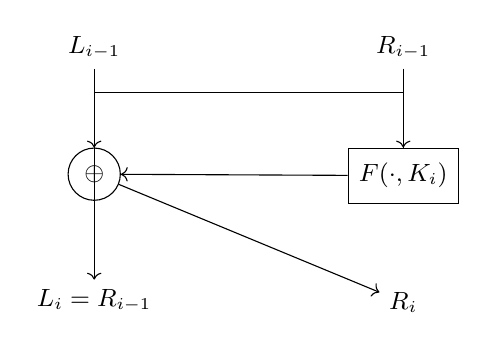
\begin{tikzpicture}[node distance=1.2cm, every node/.style={font=\small}]
  \node (Lin) {$L_{i-1}$};
  \node (Rin) [right=3cm of Lin] {$R_{i-1}$};
  \node (F) [below=1cm of Rin, draw, minimum width=1.4cm, minimum height=0.7cm] {$F(\cdot,K_i)$};
  \node (xor) [below=1cm of Lin, draw, circle, minimum size=0.6cm] {$\oplus$};
  \node (Lout) [below=1cm of xor] {$L_i = R_{i-1}$};
  \node (Rout) [below=1cm of F] {$R_i$};
  \draw[->] (Lin) -- (xor);
  \draw[->] (Rin) -- (F);
  \draw[->] (Rin.south) -- ++(0,-0.3) -| (Lout.north);
  \draw[->] (F) -- (xor) node[midway,above]{};
  \draw[->] (xor) -- (Rout);
  \draw[-] (Rin) -- (F);
\end{tikzpicture}
\end{center}
\textbf{Key points to write:}
\begin{itemize}[noitemsep]
  \item Each round: swap the halves, and XOR the right half (after passing through round function $F$ with subkey $K_i$) into the left half.
  \item Repeated for $n$ rounds (e.g.\ DES uses 16 rounds).
  \item \textbf{Decryption} reuses the exact same structure, just with the subkeys $K_n, K_{n-1}, \dots, K_1$ applied in \textbf{reverse order} --- a major practical advantage (same circuit/code for both directions).
\end{itemize}
\end{solbox}

\newpage
%% ==========================================
\section{2020 --- Group-B Q5(c): Block Cipher vs Stream Cipher (1 mark)}
%% ==========================================

\begin{qbox}{Question --- 2020 Q5(c)}
What are the differences between a block cipher and a stream cipher? \hfill [1]
\end{qbox}

\begin{solbox}{Answer --- 2020 Q5(c)}
\begin{center}
\begin{tabular}{p{4.5cm}p{4.5cm}}
\toprule
\textbf{Block Cipher} & \textbf{Stream Cipher} \\
\midrule
Encrypts a fixed-size block of bits (e.g.\ 64/128 bits) at a time & Encrypts one bit/byte at a time as data streams in \\
Same key reused per block (with a mode of operation) & Combines plaintext with a pseudorandom keystream, typically via XOR \\
Examples: DES, AES & Example: RC4 \\
\bottomrule
\end{tabular}
\end{center}
One sentence is enough for 1 mark: ``A block cipher encrypts fixed-size blocks of data at once, while a stream cipher encrypts data bit-by-bit (or byte-by-byte) continuously.''
\end{solbox}

\newpage
%% ==========================================
\section*{Exam Strategy Summary}
%% ==========================================

\begin{keybox}{High-Yield Checklist for Symmetric/Asymmetric \& Block/Stream Ciphers}
\begin{enumerate}[noitemsep]
  \item \textbf{5 ingredients of a symmetric cipher} --- plaintext, algorithm, secret key, ciphertext, decryption algorithm (1 mark each if listed, full marks if briefly explained).
  \item \textbf{Block vs stream cipher} --- one-line: "fixed block at once" vs "bit/byte-by-byte continuously". Quick 1-mark win, asked in 2020.
  \item \textbf{Classical Feistel structure} --- $L_i=R_{i-1}$, $R_i=L_{i-1}\oplus F(R_{i-1},K_i)$, plus "same structure decrypts with reversed subkeys". Shared with DES cheat sheet (\#13) --- learn once, use twice.
  \item \textbf{Public-key cryptosystem} --- 6 elements (plaintext, algorithm, public key, private key, ciphertext, decryption algorithm) + key roles ("public locks, private unlocks").
  \item \textbf{Symmetric vs asymmetric (overlap with Topic 2)} --- one shared key vs key pair; asymmetric solves key-distribution + enables signatures.
  \item This whole topic is \textbf{definition/diagram recall}, no numericals --- a 15-20 minute cheat-sheet pass should cover it cold.
\end{enumerate}
\end{keybox}

\end{document}
